\documentclass[dutch]{ucll-slides}
\usepackage{pxfonts}
\usepackage{tikz}
\usepackage{calc}
\usepackage{ucll-code}
\usepackage{siunitx}


\usetikzlibrary{calc,shadows,tikzmark,shapes.multipart,math}

\coursename{Scripttalen}
\title{Lambda's}

\newcommand{\nonterminal}[1]{{\color{red} \ensuremath{\langle}#1\ensuremath{\rangle}}}

\newenvironment{matchexamples}{
  \begin{center}
  \newcommand{\sep}{\hspace{5mm}}
  \newcommand{\match}[1]{\sep{\color{green!50!black} "##1"}}
  \newcommand{\mismatch}[1]{\sep{\color{red} "##1"}}
}{\end{center}}




\begin{document}

\maketitle

\begin{frame}
  \frametitle{Recept: Versie 1}
  \begin{overprint}
    \onslide<1>
    \code[width=.9\linewidth]{recipe-java.txt}
    \onslide<2>
    \code[width=.9\linewidth]{recipe-java2.txt}
    \onslide<3>
    \code[width=.9\linewidth]{recipe-java3.txt}
  \end{overprint}
\end{frame}

\begin{frame}
  \frametitle{Imperatieve Stijl}
  \begin{itemize}
    \item Imperatieve stijl
    \item Algoritme = lijst van sequenti\"ele stappen
    \item Volgorde uitvoering is van belang
    \item CPU hanteert imperatieve stijl
  \end{itemize}
\end{frame}

\begin{frame}
  \frametitle{Recept: Versie 2}
  \code[width=.9\linewidth]{recipe-haskell.txt}
\end{frame}

\begin{frame}
  \frametitle{Functionele Stijl}
  \begin{itemize}
    \item Functionele stijl
    \item Algoritme = \'e\'en grote uitdrukking
    \item Volgorde uitvoering is niet van belang
    \item Vergelijkbaar met wiskunde
  \end{itemize}
\end{frame}

\begin{frame}
  \frametitle{Gulden Middenweg}
  \code[width=.9\linewidth]{recipe-python.txt}
\end{frame}

\begin{frame}
  \frametitle{Evolutie}
  \begin{itemize}
    \item Evolutie naar combinatie van imperatief en functioneel
    \item Functionele stijl biedt veel voordelen
          \begin{itemize}
            \item Sneller leesbaar
            \item Doorgaans bugvrijer
            \item Beter te multithreaden
          \end{itemize}
    \item Python heeft imperatieve roots met functionele invloeden
  \end{itemize}
\end{frame}

\begin{frame}
  \frametitle{Evolutie}
  \begin{center}
    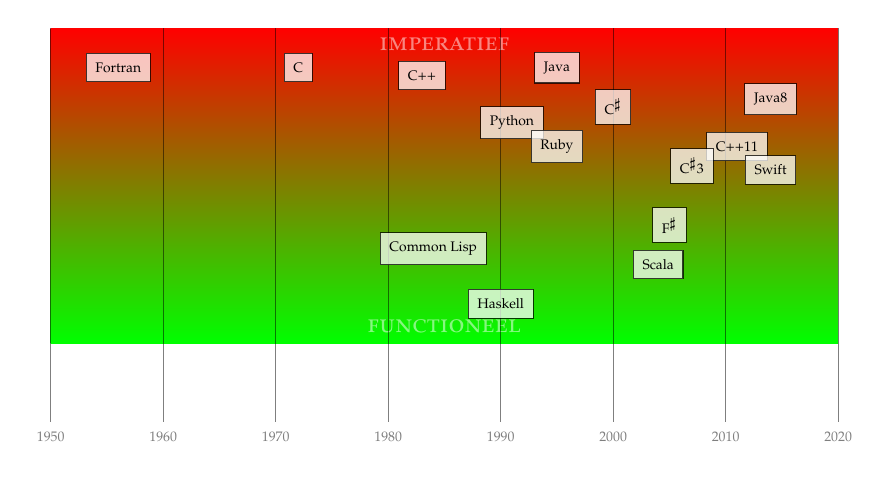
\begin{tikzpicture}[language/.style={font=\tiny,draw,fill=white,opacity=.75,text opacity=1}]
      \tikzmath{
        real \minyear;
        real \maxyear;
        int \decades;
        \minyear=1950;
        \maxyear=2020;
        \decades=int((\maxyear-\minyear)/10);
        function yeartox(\year) {
          return {(\year - \minyear)/(\maxyear - \minyear) * 10};
        };
      }
      \path[top color=red,bottom color=green] (0,-2) rectangle (10,2);
      \node[anchor=north,white,opacity=.5] at (5,2) {\scshape imperatief};
      \node[anchor=south,white,opacity=.5] at (5,-2) {\scshape functioneel};
      
      \foreach[count=\i,evaluate={\x=10/\decades*(\i-1);}] \year in {\minyear,1960,...,\maxyear} {
        \draw[thin,opacity=.5] (\x,-3) -- (\x,2) node[at start,below,font=\tiny] {\year};
      }

      \foreach[evaluate={\x=yeartox(\year)}] \language/\year/\y in {Fortran/1956/1.5,Haskell/1990/-1.5,C/1972/1.5,C++/1983/1.4,C++11/2011/0.5,Java/1995/1.5,Java8/2014/1.1,C$^\sharp$/2000/1.0,C$^\sharp$3/2007/0.25,Python/1991/0.8,Ruby/1995/0.5,F$^\sharp$/2005/-0.5,Swift/2014/0.2,Scala/2004/-1,Common Lisp/1984/-0.8} {
        \node[language] at (\x,\y) {\language};
      }
      
    \end{tikzpicture}
  \end{center}
\end{frame}

%%% Local Variables:
%%% mode: latex
%%% TeX-master: "lambdas"
%%% End:


\begin{frame}
  \frametitle{Werkvoorbeeld}
  \code[language=python]{person.py}
\end{frame}

% \input{aux-selecties.tex}
% \section{Projecties}

\frame{\tableofcontents[currentsection]}

\begin{frame}
  \frametitle{Opvragen Namen}
  \begin{quote}
    Gegeven een lijst \texttt{Person}s, wat zijn hun namen?
  \end{quote}
  \code[language=python]{getNames.py}
\end{frame}

\begin{frame}
  \frametitle{Opvragen Leeftijden}
  \begin{quote}
    Gegeven een lijst \texttt{Person}s, wat zijn hun leeftijden?
  \end{quote}
  \code[language=python]{getAges.py}
\end{frame}

\begin{frame}
  \frametitle{Veralgemening: \texttt{getFields}}
  \code[language=python,font=\small,width=.9\linewidth]{getFields.py}
  \begin{itemize}
    \item \texttt{getattr} kan gebruikt worden om waarde veld op te vragen
    \item \texttt{get\_fields} werkt op alle types objecten
    \item \texttt{get\_fields} werkt voor alle veldnamen
  \end{itemize}
\end{frame}

\begin{frame}
  \frametitle{Opvragen BMIs}
  \begin{quote}
    Gegeven een lijst \texttt{Person}s, wat zijn hun BMI's?
  \end{quote}
  \code[language=python,font=\small,width=.95\linewidth]{getBMIs.py}
  \begin{itemize}
    \item \texttt{get\_fields} werkt \emph{enkel} op velden
    \item Bewerkingen nodig $\rightarrow$ weer terugvallen op manuele lus
  \end{itemize}
\end{frame}

\begin{frame}
  \frametitle{Wat Als\dots}
  \begin{itemize}
    \item Zou handig zijn indien Python een {\tt map} lus aanbood
  \end{itemize}
  \code[language=python,font=\small,width=.9\linewidth,extra keywords={map}]{map-loop.py}
  \begin{itemize}
    \item Willekeurige bewerkingen op willekeurige objecten
  \end{itemize}
\end{frame}

%%% Local Variables:
%%% mode: latex
%%% TeX-master: "lambdas"
%%% End:

% \section{Andere ``Lussen''}

\frame{\tableofcontents[currentsection]}

\begin{frame}
  \frametitle{Tellen Van Volwassenen}
  \begin{quote}
    Tel het aantal volwassen personen.
  \end{quote}
  \vskip5mm
  \begin{overprint}
    \onslide<1>
    \code[language=python]{countAdults.py}

    \onslide<2>
    \code[language=python3, extra keywords={count}]{count-loop.py}
  \end{overprint}
\end{frame}

\begin{frame}
  \frametitle{Is Iedereen Volwassen?}
  \begin{quote}
    Zijn alle \texttt{Person}s in de lijst volwassen?
  \end{quote}
  \vskip5mm
  \begin{overprint}
    \onslide<1>
    \code[language=python]{allAdults.py}

    \onslide<2>
    \code[language=python3, extra keywords={all}]{all-loop.py}
  \end{overprint}
\end{frame}

\begin{frame}
  \frametitle{Is Er Een Volwassene?}
  \begin{quote}
    Is er minstens \'e\'en \texttt{Person} uit de lijst volwassen?
  \end{quote}
  \vskip5mm
  \begin{overprint}
    \onslide<1>
    \code[language=python]{anyAdults.py}

    \onslide<2>
    \code[language=python3, extra keywords={any}]{any-loop.py}
  \end{overprint}
\end{frame}

\section{First Class Functions}

\frame{\tableofcontents[currentsection]}

\begin{frame}
  \frametitle{Potenti\"ele Nieuwe Lussen}
  \structure{In Voorgaande Voorbeelden}
  \begin{itemize}
    \item \texttt{filter}
    \item \texttt{map}
    \item \texttt{count}
    \item \texttt{all}
    \item \texttt{any}
  \end{itemize}
  \begin{center} \itshape
    Kunnen we  deze lussen zelf implementeren?
  \end{center}
  \visible<2->{
    \begin{center}
      Ja!
    \end{center}
  }
\end{frame}

\begin{frame}
  \frametitle{\texttt{filter} Als Functie: Stapsgewijze Opbouw}
  \begin{overprint}
    \onslide<1>
    \code[language=python3,font=\small]{selectAdults2.py}
    \codeunderline{selectAdults start}{selectAdults end}

    \onslide<2>
    \code[language=python3,font=\small]{selectAdults3.py}
    \codeunderline[name center=selectAdults2 center 1]{selectAdults2 start1}{selectAdults2 end1}
    \codeoverline[name center=selectAdults2 center 2]{selectAdults2 start2}{selectAdults2 end2}
    \tikz[remember picture,overlay] \draw[thick,red,-latex] let \p1=(selectAdults2 center 2), \p2=(selectAdults2 center 1) in (\p1) -- ++(0,0.1) -- ++(2.5,0) |- ($ (\p2) + (0,-0.4) $) -- (\p2);

    \onslide<3>
    \code[language=python3,font=\small]{selectAdults4.py}
    \codeunderline[name center=selectAdults3 center 1]{selectAdults3 start1}{selectAdults3 end1}
    \codeoverline[name center=selectAdults3 center 1b,stroke/.style={thick,blue}]{selectAdults3 start1}{selectAdults3 end1}
    \codeoverline[name center=selectAdults3 center 2]{selectAdults3 start2}{selectAdults3 end2}
    \codeoverline[name center=selectAdults3 center 3,stroke/.style={thick,blue}]{selectAdults3 start3}{selectAdults3 end3}
    \tikz[remember picture,overlay] \draw[thick,red,-latex] let \p1=(selectAdults3 center 2), \p2=(selectAdults3 center 1) in (\p1) -- ++(0,0.5) |- ($ (\p2) + (0,-0.4) $) -- (\p2);
    \tikz[remember picture,overlay] \draw[thick,blue,-latex] let \p1=(selectAdults3 center 3), \p2=(selectAdults3 center 1b) in (\p1) -- ++(0,0.1) -- ++(3,0) |- ($ (\p2) + (0,0.3) $) -- (\p2);
  \end{overprint}
\end{frame}

\begin{frame}
  \frametitle{\texttt{map} Als Functie}
  \begin{overprint}
    \onslide<1>
    \code[language=python3,font=\small]{getAges2.py}
    \codeoverline{getAges2 start}{getAges2 end}

    \onslide<2>
    \code[language=python3,font=\small]{getAges3.py}
    \codeunderline[name center=getAges3 center 1]{getAges3 start1}{getAges3 end1}
    \codeoverline[name center=getAges3 center 2]{getAges3 start2}{getAges3 end2}
    \tikz[remember picture,overlay] \draw[thick,red,-latex] let \p1=(getAges3 center 2), \p2=(getAges3 center 1) in (\p1) -- ++(0,1) |- ($ (\p2) + (0,-0.4) $) -- (\p2);

    \onslide<3>
    \code[language=python3,font=\small]{getAges4.py}
    \codeunderline[name center=getAges4 center 1]{getAges4 start1}{getAges4 end1}
    \codeoverline[name center=getAges4 center 1b,stroke/.style={thick,blue}]{getAges4 start1}{getAges4 end1}
    \codeoverline[name center=getAges4 center 2]{getAges4 start2}{getAges4 end2}
    \codeoverline[name center=getAges4 center 3,stroke/.style={thick,blue}]{getAges4 start3}{getAges4 end3}
    \tikz[remember picture,overlay] \draw[thick,red,-latex] let \p1=(getAges4 center 2), \p2=(getAges4 center 1) in (\p1) |- ($ (\p2) + (0,-0.4) $) -- (\p2);
    \tikz[remember picture,overlay] \draw[thick,blue,-latex] let \p1=(getAges4 center 3), \p2=(getAges4 center 1b) in (\p1) -- ++(0,0.1) -- ++(5,0) |- ($ (\p2) + (0,0.3) $) -- (\p2);
  \end{overprint}
\end{frame}

\begin{frame}
  \frametitle{First Class Functions}
  \begin{itemize}
    \item In Python zijn functies ``first class citizens''
          \begin{itemize}
            \item Mogelijk om functies mee te geven als argument
            \item Mogelijk om functies te returnen
            \item Mogelijk om functies in variabelen te bewaren
          \end{itemize}
    \item Een functie is een object
    \item Operatie \texttt{()} dient om functie op te roepen
  \end{itemize}
  \code[language=python3,font=\small]{first-class-function.py}
\end{frame}

\begin{frame}
  \frametitle{Bestaande Functies}
  \code[language=python]{map.py}
\end{frame}

\begin{frame}
  \frametitle{Bestaande Functies}
  \code[language=python]{filter.py}
\end{frame}

\begin{frame}
  \frametitle{Bestaande Functies}
  \code[language=python]{any.py}
\end{frame}

\begin{frame}
  \frametitle{Bestaande Functies}
  \code[language=python]{all.py}
\end{frame}


%%% Local Variables:
%%% mode: latex
%%% TeX-master: "lambdas"
%%% End:

% \input{aux-lambdas-section.tex}
% \section{List Comprehensions}

\frame{\tableofcontents[currentsection]}

\begin{frame}
  \frametitle{List Comprehensions}
  \begin{itemize}
    \item {\tt map} en {\tt filter} worden vaak gebruikt
    \item Python biedt specifieke syntax
  \end{itemize}
  \vskip5mm
  \begin{overprint}
    \onslide<1>
    \code[language=python,font=\small,width=.98\linewidth]{list-comprehension.py}
    \onslide<2>
    \code[language=python,font=\small,width=.98\linewidth]{list-comprehension2.py}
  \end{overprint}
\end{frame}


%%% Local Variables:
%%% mode: latex
%%% TeX-master: "lambdas"
%%% End:


\end{document}


%%% Local Variables: 
%%% mode: latex
%%% TeX-master: t
%%% End: 
